\documentclass{sig-alternate}
%\usepackage[latin1]{inputenc} % Windows
\usepackage[utf8x]{inputenc} % Linux (unicode package needed)
% \usepackage[applemac]{inputenc} % Mac

\usepackage{hyperref}

\usepackage{balance}

\usepackage{graphicx}
\usepackage{caption}
\usepackage{subcaption}
\usepackage{hyperref}

\usepackage{xcolor}
\usepackage{color}

\newcommand{\brand}[1]{\textbf{\tt #1}}

\usepackage{enumitem}
\setlist[description]{leftmargin=*}

\definecolor{editorGray}{rgb}{0.95, 0.95, 0.95}
\definecolor{editorOcher}{rgb}{1, 0.5, 0} % #FF7F00 -> rgb(239, 169, 0)
\definecolor{editorGreen}{rgb}{0, 0.5, 0} % #007C00 -> rgb(0, 124, 0)
\colorlet{punct}{red!60!black}
\definecolor{background}{HTML}{F5F5F5}
\definecolor{delim}{RGB}{20,105,176}
\colorlet{numb}{magenta!60!black}

\usepackage{upquote}
\usepackage{listings}
\lstdefinelanguage{JavaScript}{
  morekeywords={typeof, new, true, false, catch, function, return, null, catch, switch, var, if, in, while, do, else, case, break},
  morecomment=[s]{/*}{*/},
  morecomment=[l]//,
  morestring=[b]",
  morestring=[b]'
}

\lstdefinelanguage{HTML5}{
        language=html,
        sensitive=true, 
        alsoletter={<>=-},
        otherkeywords={
                % HTML tags
        <h1>,</h1>,
        <h2>,</h2>,
        <h3>,</h3>,
        <div>,</div>,
        <a, *>, </a>,
        <html>, <head>, <title>, </title>, <meta, />, </head>, <body>,
        <canvas, \/canvas>, <script>, </script>, </body>, </html>, <!, html>, <style>, </style>, ><,
        %Web Components
        <x-route, \/x-route>,
        <api-collection-schema, \/api-collection-schema>,
        <api-collection-post, \/api-collection-post>,
        <api-collection-get, \/api-collection-get>,
        <api-collection-where, \/api-collection-where>,
        <api-model-get, \/api-model-get>,
        <api-model-put, \/api-model-put>,
        <api-model-del, \/api-model-del>,
        <x-input, \/x-input>,
        <x-form,  \/x-from>,
        <x-table, \/x-table>,
        <x-pager, \/x-pager>,
        <x-router>, <\/x-router>,
        <template, *>, </template>
        },  
        ndkeywords={
        % General
        =,
        % HTML attributes
        charset=, id=, width=, height=,
        % CSS properties
        border:, transform:, -moz-transform:, transition-duration:, transition-property:, transition-timing-function:,
        %custom
        content
        },  
        morecomment=[s]{<!--}{-->},
        tag=[s]
}

\lstset{%
    % Basic design
    backgroundcolor=\color{background},
    basicstyle={\scriptsize\ttfamily},   
    frame=none,
    % Line numbers
    numbers=none,
    % xleftmargin={0.75cm},
    % numbers=left,
    % stepnumber=1,
    % firstnumber=1,
    % numberfirstline=true,
    % Code design   
    keywordstyle=\color{blue}\bfseries,
    commentstyle=\color{darkgray}\ttfamily,
    ndkeywordstyle=\color{editorGreen}\bfseries,
    stringstyle=\color{delim},
    % Code
    language=HTML5,
    alsolanguage=JavaScript,
    alsodigit={.:;},
    tabsize=2,
    showtabs=false,
    showspaces=false,
    showstringspaces=false,
    extendedchars=true,
    breaklines=true,        
    % Support for German umlauts
    literate=%
    {Ö}{{\"O}}1
    {Ä}{{\"A}}1
    {Ü}{{\"U}}1
    {ß}{{\ss}}1
    {ü}{{\"u}}1
    {ä}{{\"a}}1
    {ö}{{\"o}}1
}

\lstdefinelanguage{json}{
    basicstyle=\scriptsize\ttfamily,
    % Line numbers
    numbers=none,
    frame=none,
    % numbers=left,
    % numberstyle=\scriptsize,
    % stepnumber=1,
    % numbersep=8pt,
    % showstringspaces=false,
    % breaklines=true,
    % frame=lines,
    backgroundcolor=\color{background},
    literate=
     *{0}{{{\color{numb}0}}}{1}
      {1}{{{\color{numb}1}}}{1}
      {2}{{{\color{numb}2}}}{1}
      {3}{{{\color{numb}3}}}{1}
      {4}{{{\color{numb}4}}}{1}
      {5}{{{\color{numb}5}}}{1}
      {6}{{{\color{numb}6}}}{1}
      {7}{{{\color{numb}7}}}{1}
      {8}{{{\color{numb}8}}}{1}
      {9}{{{\color{numb}9}}}{1}
      {:}{{{\color{punct}{:}}}}{1}
      {,}{{{\color{punct}{,}}}}{1}
      {\{}{{{\color{delim}{\{}}}}{1}
      {\}}{{{\color{delim}{\}}}}}{1}
      {[}{{{\color{delim}{[}}}}{1}
      {]}{{{\color{delim}{]}}}}{1},
}

\begin{document}

% Copyright
\setcopyright{acmcopyright}
%\setcopyright{acmlicensed}
%\setcopyright{rightsretained}
%\setcopyright{usgov}
%\setcopyright{usgovmixed}
%\setcopyright{cagov}
%\setcopyright{cagovmixed}


% DOI
\doi{10.475/123_4}

% ISBN
\isbn{123-4567-24-567/08/06}

%Conference
\conferenceinfo{DocEng2015}{Sep 8--11, 2015, Lausanne, Switzerland}

\acmPrice{\$15.00}

\title{x-project: a document-oriented toolkit to design and implement Web Applications based on HTML5 Web Components}

\numberofauthors{4} 
\author{
\alignauthor
Andrea D'Amelio\\
  \affaddr{Universit\`a Roma Tre}\\
  \affaddr{Dipartimento di Ingegneria}\\
  \affaddr{Universit\`a Roma Tre}\\
  \affaddr{Rome, Italy}\\
  \email{damelio@ing.uniroma3.it}
\alignauthor
Enrico Marino\\
  \affaddr{Universit\`a Roma Tre}\\
  \affaddr{Dipartimento di Ingegneria}\\
  \affaddr{Universit\`a Roma Tre}\\
  \affaddr{Rome, Italy}\\
  \email{marino@ing.uniroma3.it}
\and
\alignauthor
Tiziano Sperati\\
  \affaddr{Universit\`a Roma Tre}\\
  \affaddr{Dipartimento di Ingegneria}\\
  \affaddr{Universit\`a Roma Tre}\\
  \affaddr{Rome, Italy}\\
  \email{sperati@ing.uniroma3.it}
\alignauthor
Federico Spini\\
  \affaddr{Universit\`a Roma Tre}\\
  \affaddr{Dipartimento di Ingegneria}\\
  \affaddr{Universit\`a Roma Tre}\\
  \affaddr{Rome, Italy}\\
  \email{spini@ing.uniroma3.it}
}

\maketitle

\begin{abstract}
This work introduces the \brand{x-project} toolkit, a software library essentially composed by a collection of Web Components based on \href{https://www.polymer-project.org}{Polymer Project} by Google. The toolkit is then applied along with a modern web framework, namely \href{http://loopback.io/}{Loopback} by Strongloop, to realize an hybrid prototypal tool which brings together the customizability of a modern web framework with the ease of use of traditional CMSs.

Furthermore, the toolkit usage implicitly defines a document-driven development process that leads to a very readable, maintainable and extensible code by imposing a neat logic decomposition that strongly supports an engineered design of the web application.
\end{abstract}


%
% The code below should be generated by the tool at
% http://dl.acm.org/ccs.cfm
% Please copy and paste the code instead of the example below. 
%

\begin{CCSXML}
<ccs2012>
<concept>
<concept_id>10011007.10011006.10011066</concept_id>
<concept_desc>Software and its engineering~Development frameworks and environments</concept_desc>
<concept_significance>500</concept_significance>
</concept>
<concept>
<concept_id>10011007.10011074.10011092</concept_id>
<concept_desc>Software and its engineering~Software development techniques</concept_desc>
<concept_significance>500</concept_significance>
</concept>
<concept>
<concept_id>10002951.10003260.10003282</concept_id>
<concept_desc>Information systems~Web applications</concept_desc>
<concept_significance>300</concept_significance>
</concept>
</ccs2012>
\end{CCSXML}

\ccsdesc[500]{Software and its engineering~Development frameworks and environments}
\ccsdesc[500]{Software and its engineering~Software development techniques}
\ccsdesc[300]{Information systems~Web applications}

%
% End generated code
%

%
%  Use this command to print the description
%
\printccsdesc

\section{Introduction}\label{sec:introduction}








Lorem ipsum dolor sit amet, consectetur adipisicing elit, sed do eiusmod
tempor incididunt ut labore et dolore magna aliqua. Ut enim ad minim veniam,
quis nostrud exercitation ullamco laboris nisi ut aliquip ex ea commodo
consequat. Duis aute irure dolor in reprehenderit in voluptate velit esse
cillum dolore eu fugiat nulla pariatur. Excepteur sint occaecat cupidatat non
proident, sunt in culpa qui officia deserunt mollit anim id est laborum.


Section 2 presents the context where \brand{x-project} is positioned, overviewing the CMS evolution; section 3 introduces \brand{x-project}, its philosophy and architecture. Section 4 shows a case study in which is implemented a blog using x-project toolkit. Finally, section 5 draws conclusions.


One generally accepted definition of Content Management System is: a system that lets you apply management principles to content.

It is simple to elicit an evolutionary path in the history of management systems whose milestones are identifiable in \emph{Joomla!}, \emph{Wordpress} and \emph{KeystoneJS}.

Alongside these milestones entire constellations of analogous experiences popped up, but we considered them not relevant since they borrowed main features and constitutive approaches from cited ones. 

Starting from \emph{Joomla!}, a framework that drove in the engineering into the world of web content management. Joomla! powers more than 2,7\% of the largest 1,000,000 web sites in the world \cite{usage-cms}. Anyway, nowadays, \emph{Joomla!} results unwieldy and, due to its monolithic approach, not complied to current web features.

\emph{Wordpress}, instead is used by more than 23.3\% of the top 10 million websites (as of January 2015) \cite{usage-cms}. Wordpress develop CMS’s idea, driving in the intention to use CMSs to build Web Application. Wordpress, with its plugin, aims to limber user experience. The availability of more than 37,000 plugins, because it lets to create sites to non-experts too.
Anyway, further customizations, other than the ones introduced by plugins, are difficult to deploy due to loosely code engeneering of this tool.

Finally, {\em KeystoneJS} stand in the last position. Minimal and agile, KeystoneJS, embody the new era of the CMS, letting the user to make his own personal web application.



KeystoneJS





The remainder of this document is organized as follows. In
Section~\ref{sec:cycle} we provide an overview of the proposed web development cyle process. Section~\ref{sec:architecture} is devoted to describe the architecture and the tecnology stack exposed by applications developed with the toolkit, while section~\ref{sec:toolkit} presents the toolkit itself. Section~\ref{sec:case-study} reports about a case-study application of the toolkit discussed in this paper. Finally, Section~\ref{sec:conclusions} proposes some conclusive remarks and future developments.




%%% ----

% To speed up web application development, frameworks mostly rely on external configuration files and less on procedural code \cite{6859693}.


\section{Architecture}\label{sec:architecture}

A Web application developed exploiting the \brand{x-project} toolkit, an \brand{x-project} app, is a full stack {\em JavaScript} Single Page Application.

\paragraph{Server side}

On the server-side, an \brand{x-project} app is based on:

\begin{description}
\itemsep1pt\parskip0pt\parsep0pt
\item[StrongLoop LoopBack] generates model API from the models schemas, to let CRUD operations on models.
These schemas are JSON documents. Each document represents a model and presents the following fields: the \texttt{name} of the model, the set of \texttt{properties}, the list of \texttt{relations} to others models and the list of \texttt{ACL} (Access Control Layer) rules. 
The API can be extended: the developer can add remote functions to models or add hooks to existing API to add custom behavior before and/or after the API handler (to pre-process the request and/or post-process the response). 
The resulting API is RESTful, cookie free, signed by authentication token.
By default, applications have a built-in model that represent a user, with properties \texttt{username}, \texttt{email} and \texttt{password} for login and the property \texttt{role} used by the ACL module.
{\em Loopback} also introduces an indirection layer that allows to choose among (almost) any particular DBMS to use.
\end{description}

\paragraph{Client side}

On the client-side, an \brand{x-project} app is based on:

\begin{description}
\itemsep1pt\parskip0pt\parsep0pt

\item[Web Components] are an umbrella term for four different W3C specifications \cite{w3c}:
\emph{Custom Elements} to define custom HTML elements;
\emph{HTML Templates} to define blocks of markup with the ability to inject dynamic content into;
\emph{Shadow DOM} to scope markup and styles in a separate DOM tree;
\emph{HTML Imports} to include and reuse HTML documents in other HTML documents.
Each of these pieces is useful individually. But when combined, this whole package offers:
\emph{Composability}, being able to create whole sites and apps by putting different elements together;
\emph{Encapsulation}, isolating markup, style, and behavior logic so they don't leak into the rest of the page;
\emph{Reusability}, extending existing elements to create new elements, allowing to stop reinventing the wheel.
This brings a less fragmented ecosystem, where components can truly interoperate with each other.
Since these specifications are currently W3C Working Draft, they aren't fully supported across all major browsers. \texttt{webcomponents.js} is a set of polyfills built on top of the Web Components specifications. 
As these technologies are implemented in browsers, the polyfills will shrink to gain the benefits of native implementations \cite{webcomponents-polyfills}. 
        
\item[Polymer library] (\url{https://www.polymer-project.org/}) provides a thin layer of API on top of Web Components and several powerful features, such as custom events and delegation, mixins, accessors and component life-cycle functions, to facilitate the creation of Web Components. 
%Similar to \emph{Polymer} are \emph{x-tag} and \emph{Bosonic}. 
%Web repositories \url{http://component.kitchen} and \url{http://customelements.io} already counts thousands of open source user-contributed custom elements.
\end{description}

% \begin{figure}[!htbp]
% \centering
% 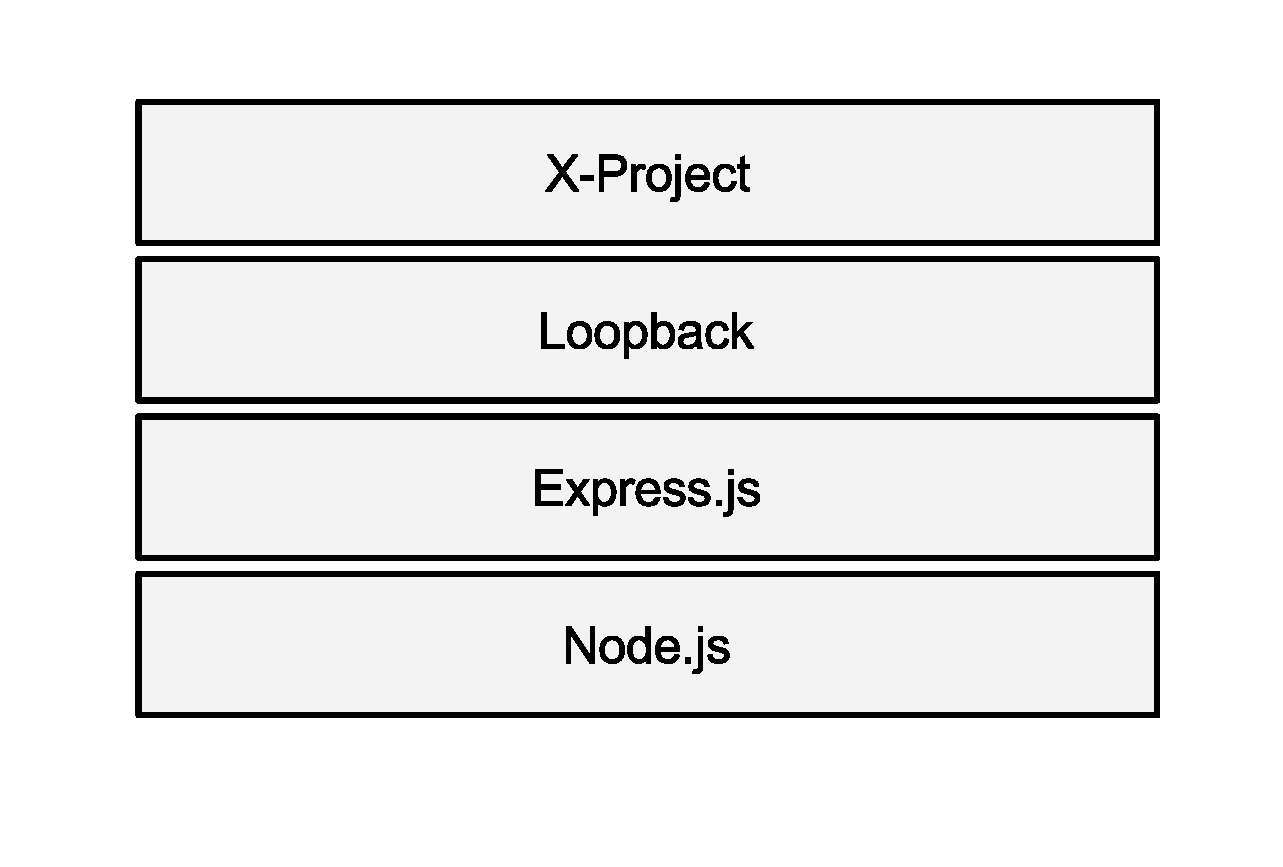
\epsfig{file=images/stack.eps, height=0.2\textwidth}
% \caption{Technology stack}
% \label{fig:tech-stack}
% \end{figure}

% \begin{figure}[!h]
%  \centering
%  \begin{subfigure}[b]{0.53\linewidth}
%  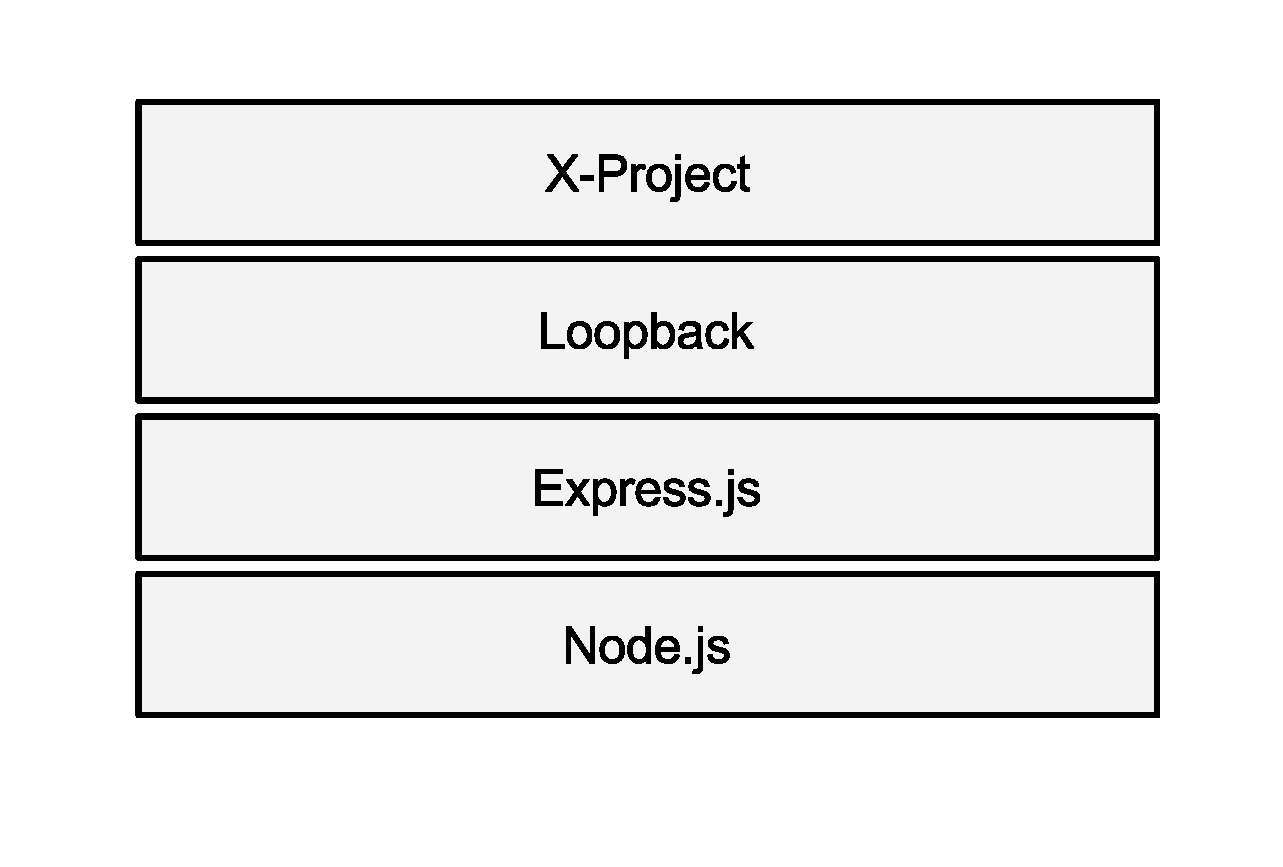
\includegraphics[width=\textwidth]{images/stack.eps} 
%  \caption{Technology stack.}
%  \label{fig:tech-stack}
%  \end{subfigure}
%  ~
%  \begin{subfigure}[b]{0.43\linewidth}
%  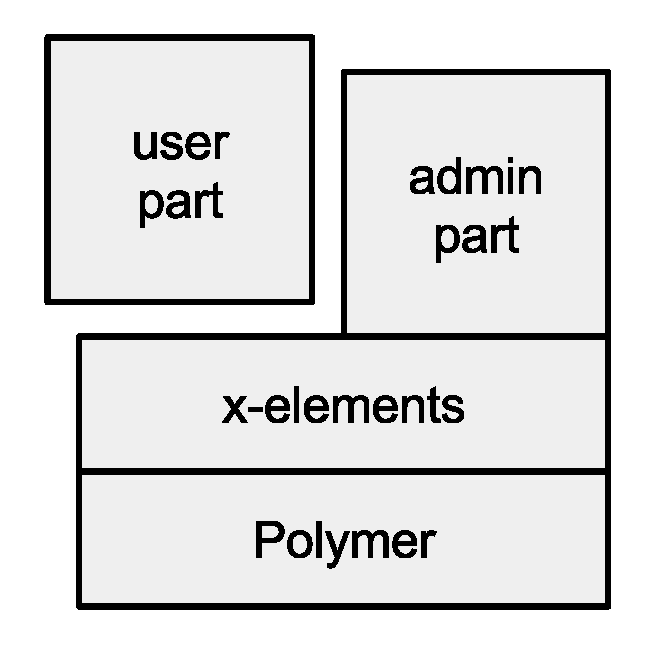
\includegraphics[width=\textwidth]{images/client-arch.eps}
%  \caption{Client-side architecture}
%  \label{fig:client-arch}
%  \end{subfigure}
 
%  % \caption{Office building: 
%  % (a) the schematic plan; 
%  % (b) the simplified 3D model generated for testing on the field 
%  % the indoor mapping project described in this paper.
%  % }
%  % \label{fig:sogei}
% \end{figure}

% \begin{figure}[!htbp]
% \centering
% 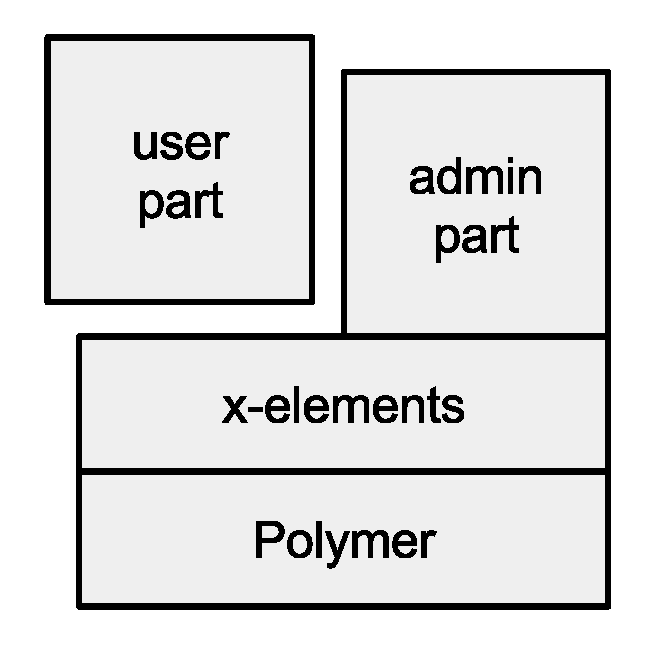
\epsfig{file=images/client-arch.eps, height=0.2\textwidth}
% \caption{Client-side architecture}
% \label{fig:client-arch}
% \end{figure}



\section{x-project toolkit}\label{sec:toolkit}

``Everything is an element'', from an AJAX request to an entire web page. Every part of the website is encapsulated inside an element. 

\brand{x-project} provides a set of Polymer elements for local routing, API requests, forms, lists, style and admin pages, as listed below \footnote{\scriptsize For the sake of conciseness, Polymer Elements are presented as empty elements, although empty element type is not supported. Furthermore, template variable are enclosed in single curly brackets while Polymer requires double curly brackets.}. 

Elements can be customized through their attributes. 

Attributes can act as inputs parameters (values having effects on the element) or output parameters (values that are returned by the element).
Values in parameters could be hard-coded (if they never change) or stored in variables.
Different parameters in different elements could use the same variable, so, the value of an output parameter of an element could be used as input in an input parameter of another element.

\paragraph{Elements for local routing}

The following elements perform local routing (for Single Page Application).

\vspace{0.2cm}

\texttt{<x-router>} implements local routing using \emph{HTML5 Push State API}. It represents the core element of the app. It intercepts routes, creates pages, and passes parameters to the page.

\vspace{0.2cm}

\texttt{<x-route>} represents a route-to-page mapping. 
Parameters presented in an URL are sent as attributes to the corresponding page.

\begin{lstlisting}[language=HTML5]
<x-route route="{route}" page="{page}" />
\end{lstlisting}

\texttt{<x-link>} is an extension of the anchor element \texttt{<a>} that prevents the default behavior when a click event occurs, blocking page request to the server and redirecting the request to the local router. 

\begin{lstlisting}[language=HTML5]
<a is="x-link" href="{href}">{link}</a>
\end{lstlisting}

\paragraph{Elements for API management}

The following elements handle HTTP RESTful API for the collections of the app.

\texttt{<api-collection-schema>} gets the schema of a collection. 

\begin{lstlisting}[language=HTML5]
<api-collection-schema name="{collection}" 
  schema="{schema}" />
\end{lstlisting}

\vspace{0.2cm}

\texttt{<api-collection-post>} creates a model of a collection. 

\begin{lstlisting}[language=HTML5]
<api-collection-post 
  name="{name}" model="{model}" />
\end{lstlisting}

\vspace{0.2cm}

\texttt{<api-collection-get>} gets models of a collection. 

\begin{lstlisting}[language=HTML5]
<api-collection-get 
  name="{collection}" where="{where}" 
  page="{page}" perpage="{perpage}"  
  items="{items}" count="{count}" />
\end{lstlisting}

Where: 
\texttt{name} is the name of the collection to retrieve; 
\texttt{where} is an object that specifies a set of logical conditions to match, similar to a \texttt{WHERE} clause in a SQL query;
\texttt{page} and \texttt{perpage} are parameters for the pagination;
\texttt{items} are the retrieved models that match the query composed by the \texttt{where} clause and the pagination parameters;
\texttt{count} is the size of the collection (the total number of items of the collection).

\vspace{0.2cm}

\texttt{<api-collection-where>} dynamically generates a form from a model schema, to create an API \texttt{where} clause filter. Specifically, for each property described in the model schema, it generates a corresponding input filter field. 

\begin{lstlisting}[language=HTML5]
<api-collection-where schema="{schema}"
  where="{where}" />
\end{lstlisting}

Where: \texttt{schema} is the schema of the collection (it acts as an input);
\texttt{where} is the filter object.

\vspace{0.2cm}

\texttt{<api-model-get>} retrieves a model of a collection. 

\begin{lstlisting}[language=HTML5]
<api-model-get name="{name}" model-id="{id}" 
  model="{model}" />
\end{lstlisting}

Where: 
\texttt{name} is the name of the collection of the model; 
\texttt{model-id} is the model id; 
\texttt{model} is the model retrieved (it acts as an output).

\vspace{0.2cm}

\texttt{<api-model-put>} update a model of a collection. 

\begin{lstlisting}[language=HTML5]
<api-model-put name="{name}" model-id="{id}" 
  model="{model}" />
\end{lstlisting}

Where: 
\texttt{model} is the model updated (it acts as an input).

\vspace{0.2cm}

\texttt{<api-model-del>} deletes a model of a collection. 

\begin{lstlisting}[language=HTML5]
<api-model-del name="{name}" model-id="{id}" />
\end{lstlisting}

\paragraph{Elements for forms}
The following elements are used to create forms. 

\vspace{0.2cm}

\texttt{<x-input>} is an extension of the input element. 

\begin{lstlisting}[language=HTML5]
<x-input type="{type}" label="{label}"
  value="{value}" />
\end{lstlisting}

Where: 
\texttt{type} can be \texttt{string}, \texttt{number}, \texttt{date}, \texttt{email}, \texttt{url}, \texttt{location} (with auto-completion based on Google Place API) and \texttt{file}.

\vspace{0.2cm}

\texttt{<x-form>}  dynamically generates a form from a model schema, to create/update a model.

\begin{lstlisting}[language=HTML5]
<x-form schema="{schema}" model="{model}" />
\end{lstlisting}

\paragraph{Elements for lists}

The following elements are used to manage lists. 

\vspace{0.2cm}

\texttt{<x-table>}  dynamically generates a table of models from a model schema. 

\begin{lstlisting}[language=HTML5]
<x-table schema="{schema}" items="{items}" />
\end{lstlisting}

Where \texttt{schema} is used to generate the columns of the table; 
\texttt{items} is used to generate the rows (the values) of the table.

\vspace{0.2cm}

\texttt{<x-pager>} generates the list of links to handle pagination.

\begin{lstlisting}[language=HTML5]
<x-pager perpage="{perpage}" count="{count}" 
  current="{page}" />
\end{lstlisting}

Where \texttt{count} is the total number of items to paginate; 
\texttt{perpage} is the number of items per page; 
\texttt{current} is the current page selected by the user.

By itself pagination doesn't paginate any list, but it can be used in conjunction with \texttt{<api-collection-get>} (as shown in the case study), where the \texttt{current} output parameter of \texttt{<x-pager>} is the input \texttt{page} parameter of \texttt{<api-collection-get>}.

\paragraph{Elements for style}

The style is based on \texttt{iron-flex-layout} \cite{iron-elements}, a CSS library of style mixins for cross-platform Flexible Box layouts.

\paragraph{Elements for admin pages}

Even a page can be encapsulated in an element. \brand{x-project} provides a set of pages for the admin part of the app, \texttt{<page-collection>} and \texttt{<page-model-edit>}, presented below.

% \begin{figure}[!htbp]
% \centering
% 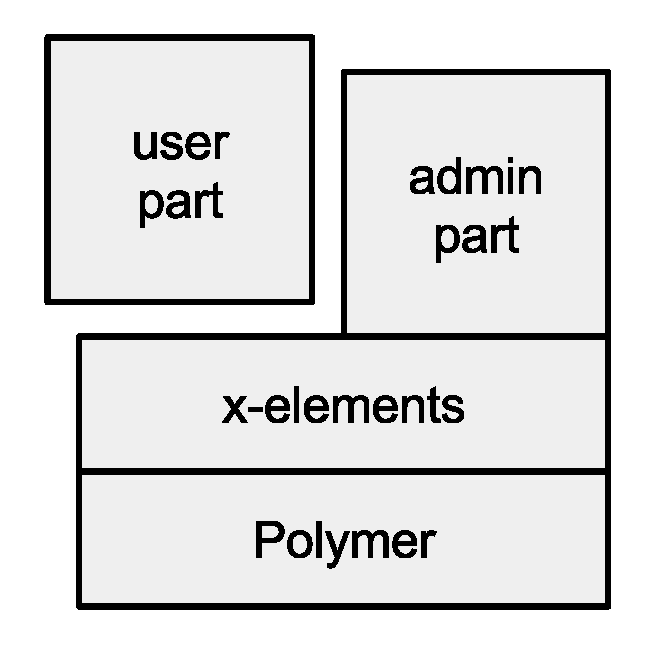
\epsfig{file=images/client-arch.eps, height=0.2\textwidth}
% \caption{Client-side architecture}
% \label{fig:client-arch}
% \end{figure}



\section{Document-driven web development process}\label{sec:dev-proc}

The process to build a web application based on \brand{x-project} toolkit consists of the following four steps.

\textbf{1\textsuperscript{st} step - Models schemas definition}. A description of entities, properties, relations and data access policies are defined as JSON documents.

\textbf{2\textsuperscript{nd} step - HTTP RESTful API definition}. CRUD operations on models are automatically generated by the web framework (on the basis of input JSON documents) and further custom actions can be defined. All of them are exposed as HTTP RESTful API.

\textbf{3\textsuperscript{rd} step - UI components definition}. Distinct UI components can be defined, or retrieved from a collection of predefined components, configured and adapted. They represent the building blocks of the whole UI.

\textbf{4\textsuperscript{th} step - UI components assembly}. Distinct UI components are finally mounted to compose the application views. Assembly is kept as simple as possible: it only consists of a composition of HTML5 elements.

\vspace{0.2cm}

So the entire development process results driven by: JSON documents describing entities of the application and HTML template documents describing the UI components.

% This modellization is based on the reasonable assumption that server side
% operation on data models are nowadays be sufficently explored, and as proven by
% the {\em KeystoneJS} experience, at least one choice is available to automagically  
% 1) generate server-side CRUD methods on models with ACL capabilities and 
% 2) handle users and sessions, 
% once a JSON description of data models and relations between them are provided to the
% system. This very JSON descriptor documents drive the whole process, actually composed
% by the following four steps.

% se avanza spazio si possono mettere dei nomignoli per ogni stepche potrebbero essere:
% 1. JSON data model description
% 2. Model actions definion
% 3. UI component definition
% 4. UI component assemplation

% PARLARE DI DECOMPOSIZIONE VERTICALE??


\section{Case study}\label{sec:case-study}
In this section the design and the implementation of a blog platform is presented. 

\paragraph{1\textsuperscript{st} step - Models schemas definition}
As to a blog platform, the essential entities to be modelled are the following: \texttt{Post} and \texttt{Tag}.

\begin{lstlisting}[language=json]
{
  "name": "Post",
  "properties": {
    "title": { "type": "string" },
    "posted": { "type": "date" },
    "content": { "type": "text" },
    "permalink": { "type": "string" }
  }, 
  "relations": {
    "tags": { "type": "has_many", "model": "Tag"}
  }
}
\end{lstlisting}

\begin{lstlisting}[language=json]
{
  "name": "Tag",
  "properties": {
    "name": { "type": "string" }
  }
}
\end{lstlisting}

\paragraph{2\textsuperscript{nd} step - HTTP RESTful API definition}
These models result in the following HTTP RESTful API (automatically generated by Loopback server).

\begin{lstlisting}
GET|POST /api/Posts
GET|PUT|DELETE /api/Posts/:post_id
GET|POST /api/Tags
GET|PUT|DELETE /api/Tags/:tag_id
\end{lstlisting} 

\paragraph{3\textsuperscript{rd} step - UI components definition}
In this simple example, there is no need to define further components besides the ones provided by the \brand{x-project} toolkit.

\paragraph{4\textsuperscript{th} step - UI components assembly}
Since a snippet is worth a thousand words, in the following the code of the pages of the app is shown.
It is important to remark how easily a page can be built without writing code but assembling elements.

Tha admin part is composed by two pages: \texttt{page-collection} and \texttt{page-model-edit}.
These pages are accessible via the following routes.

\begin{lstlisting}[language=HTML5]
<x-router>
  <x-route route="/admin/:collection" 
    page="page-collection" />
  <x-route route="/admin/:collection/:id"
    page="page-model-edit" />
</x-router>
\end{lstlisting}

Where:
the parameter \texttt{:collection} is the name of the collection to inspect;
the parameter \texttt{:id} is the id of the model to edit.
These parameters are set as attributes of the page element.

\vspace{0.2cm}

\texttt{<page-collection>} shows the models of a collection.

\begin{lstlisting}[language=HTML5]
<template name="page-collection">
  <api-collection-schema name="{collection}"
    schema="{schema}" />
  <api-collection-get 
    name="{collection}" where="{where}" 
    page="{page}" perpage="{perpage}"  
    items="{items}" count="{count}" />
  <api-collection-where schema="{schema}"
    where="{where}" />
  <x-table schema="{schema}" items="{items}" />
  <x-pager count="{count}" perpage="{perpage}"
    current="{page}" />
</template>
\end{lstlisting}

Where: 
the value \texttt{collection} is picked from the url, via the parameter \texttt{:collection};
the value \texttt{schema} is the output of \texttt{<api-collection-schema>} and the input of \texttt{<api-collection-get>} and \texttt{<x-table>};
the value \texttt{items} is the output of \texttt{<api-collection-get>} and the input of \texttt{<x-table>};
the value \texttt{where} is the output of \texttt{<api-collection-where>} and the input of \texttt{<api-collection-get>};
the value \texttt{count} is the output of \texttt{<api-collection-get>} and the input of \texttt{<x-pager>};
the values \texttt{perpage} and \texttt{page} are the outputs of \texttt{<x-pager>} and the inputs of \texttt{<api-collection-get>};
every time the user (the admin) interacts with the pagination (\texttt{<x-pager>}) or the advanced search options (\texttt{<api-collection-where>}), \texttt{<api-collection-get>} regenerates the request to get the list of models using pagination and query parameters.

\vspace{0.2cm}

\texttt{<page-model-edit>} shows the forms to update a model.

\begin{lstlisting}[language=HTML5]
<template name="page-model-edit">
  <api-collection-schema name="{collection}"
    schema="{schema}" />
  <api-model-get name="{collection}" 
    model-id="{id}" model="{model}" />
  <x-form schema="{schema}" model="{model}" />
  <api-model-put  name="{collection}"
    model-id="{id}" model="{model}" />
</template>
\end{lstlisting}

Where: 
the value \texttt{schema} is the output of \texttt{<api-collection-schema>} and the input of \texttt{<x-form>};
the value \texttt{model} is the output of \texttt{<api-model-get>} and \texttt{<x-form>} and the input of \texttt{<api-model-put>}.
Once the page is ready (initialized and served by the local router): 
\texttt{<api-collection-schema>} fetch the \texttt{schema}; 
\texttt{<api-model-get>} fetch the model (a post or a tag) identified by \texttt{id};
\texttt{<x-form>} shows the form to edit the model.
When the model changes (is updated via the form) \texttt{<api-model-put>} sends a request to the server to update the database (via the corresponding HTTP RESTful API).


The user part is essentially composed by two pages: \texttt{page-posts} and \texttt{page-post}.

\begin{lstlisting}[language=HTML5]
<x-router>
  <x-route route="/" page="page-posts" />
  <x-route route="posts/:id" page="page-post" />
</x-router>
\end{lstlisting}

\texttt{<page-posts>} shows the list of posts.

\begin{lstlisting}[language=HTML5]
<template name="page-posts">
  <api-collection-get name="Posts"
    perpage="10" page="{page}" 
    items="{posts}" count="{count}" />
  <template is="dom-repeat" items="{posts}">
    <li>{item.title} {item.date}</li>
  </template>
  <x-pager perpage="10" total="{count}" 
    current="{page}" />
</template>
\end{lstlisting}

Where:
the value \texttt{posts} is the output of \texttt{<api-collection-get>} and the input of the \texttt{<template>} iterator; for each \texttt{item} in \texttt{posts}, a list item with the post info (\texttt{title} and publishing \texttt{date}) is printed;
\texttt{<x-pager>} component is the same used in the page \texttt{<page-collection>}.

\vspace{0.2cm}

\texttt{<page-post>} shows a post. 

\begin{lstlisting}[language=HTML5]
<template name="page-post">
  <api-model-get name="Posts" model-id="{id}" 
    model="{post}" />
  <h1>{post.title}</h1>
  <h2>by {post.author}</h2>
  <h3>on {post.date}</h3>
  <div>{post.content}</div>
</template>
\end{lstlisting}

Where:
the value \texttt{post} is the output of \texttt{<api-model-get>} and it is used to compose the page.
Once \texttt{<api-model-get>} has fetched the \texttt{post} (identified by \texttt{id}),
\texttt{title}, \texttt{author}, \texttt{date} and \texttt{content} of the \texttt{post} will be shown.



%\section{Conclusion}

In the present time open source CMS has gained a big market. 
Generally all CMSs fulfill common task of content like create, edit, publish. 
Lots of varieties are available based on functionality and platform, such as \emph{good user support}, \emph{security aspects}, \emph{plug-ins ecosystem}, \emph{documentation}, etc.

\cite{6169111} propose different performance criteria like \emph{page load time}, \emph{page size}, \emph{number of request}, \emph{number of bootstrap resources files}.
 
\cite{5552271} propose about thirty features criteria that could be classified in: \emph{Admin Management}, \emph{Data Management}, \emph{User Management}, \emph{UI Management}, \emph{Web Content Management}, \emph{Multimedia Data Management}.



\bibliographystyle{abbrv}
\bibliography{x-project-paper}
\end{document}





